\section{Running Example}
\label{sec:running_example}

This section introduces the running example used in the rest of paper to illustrate how our OpenAPI to CPN transformation approach.
% 
Let us consider as an example a simple Web application (client and server) where a user logs in and checks their shopping cart. This example is taken from the OWASP Juice Shop project\footnote{Accessible in~\url{https://owasp.org/www-project-juice-shop/}}, a cybersecurity education project with an insecure Web application. This project is commonly used in security training, awareness demos, security competitions, and to test security tools. 

The UML Sequence Diagram in Figure~\ref{fig:simplesWebAPIJuiceShop} illustrates the interaction between the REST API client and the server. In the beginning, the client application initiates communication by sending a POST request with the credentials to the \texttt{/login} endpoint of the server application. The server application responds with the information related to that user, such as the basket ID (\textit{bid}) and \textit{token}. With the information received, the client application sends a new request to the server for the \texttt{/basket/<bid>} endpoint and again, the server application responds with the requested information.

The REST API in this example is vulnerable to {\em Broken Object Level Authorization}, which is ranked \#1 in the OWASP API Security Top 10 2019\footnote{Accessible in~\url{https://owasp.org/www-project-api-security/}}. Exploiting this vulnerability is quite simple. An attacker can simply send a request to the \texttt{/basket/<bid>} endpoint with a   different bid than the one given by the server in a previous request. For example, if the client requests \textit{/basket/2} in Figure~\ref{fig:simplesWebAPIJuiceShop}, the server will respond with the another user's shopping basket information. 


\begin{figure}[!htp]
    \center
    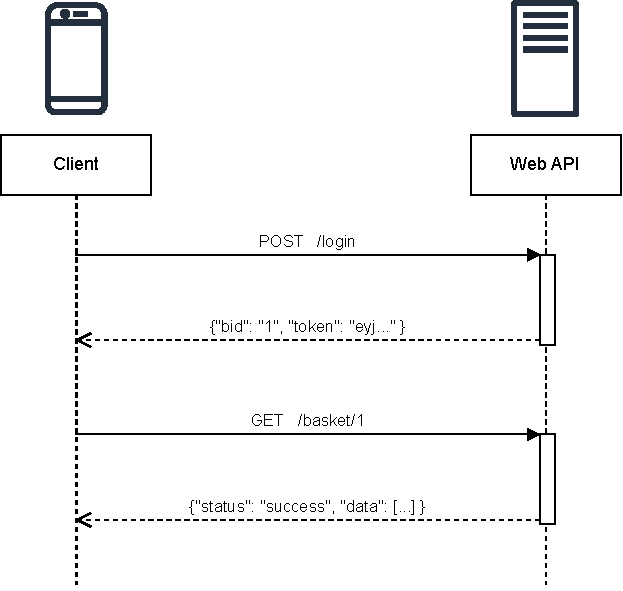
\includegraphics[width=0.9\columnwidth]{figures/SimpleJuiceShop.drawio.pdf}
    \caption{A simple WebAPI interaction.}
    \label{fig:simplesWebAPIJuiceShop}
\end{figure}

%
%
%The first step is to convert the OpenAPI specification of this API to a Colored Petri Net (this step is detailed in Section~\ref{sec:transformation}). The OpenAPI specification can be checked here\footnote{\url{https://app.swaggerhub.com/apis/ailton07/JuiceShop/1.0.0/}}.
%After applying the model transformation algorithm, explained in Section~\ref{sec:transformation}, the result obtained is as illustrated in Figure~\ref{fig:simplesWebAPIJuiceShopPetriNet-step-0}. We have the transition \textit{post-/rest/user/login-200} representing the case where the server receives a POST request to endpoint \textit{/rest/user/login} that results in a response with status code 200. We have a place \textit{bid get-/rest/basket/{bid}} that holds the information required to create a GET request to endpoint \textit{/rest/basket/{bid}}. Finally, we have the transition \textit{get-/rest/basket/{bid}-200} to represent the case where the server receives a GET request to endpoint \textit{/rest/basket/{bid}} that results in a response with status code 200.
%
%
%\begin{figure}[!htp]
%    \center
%    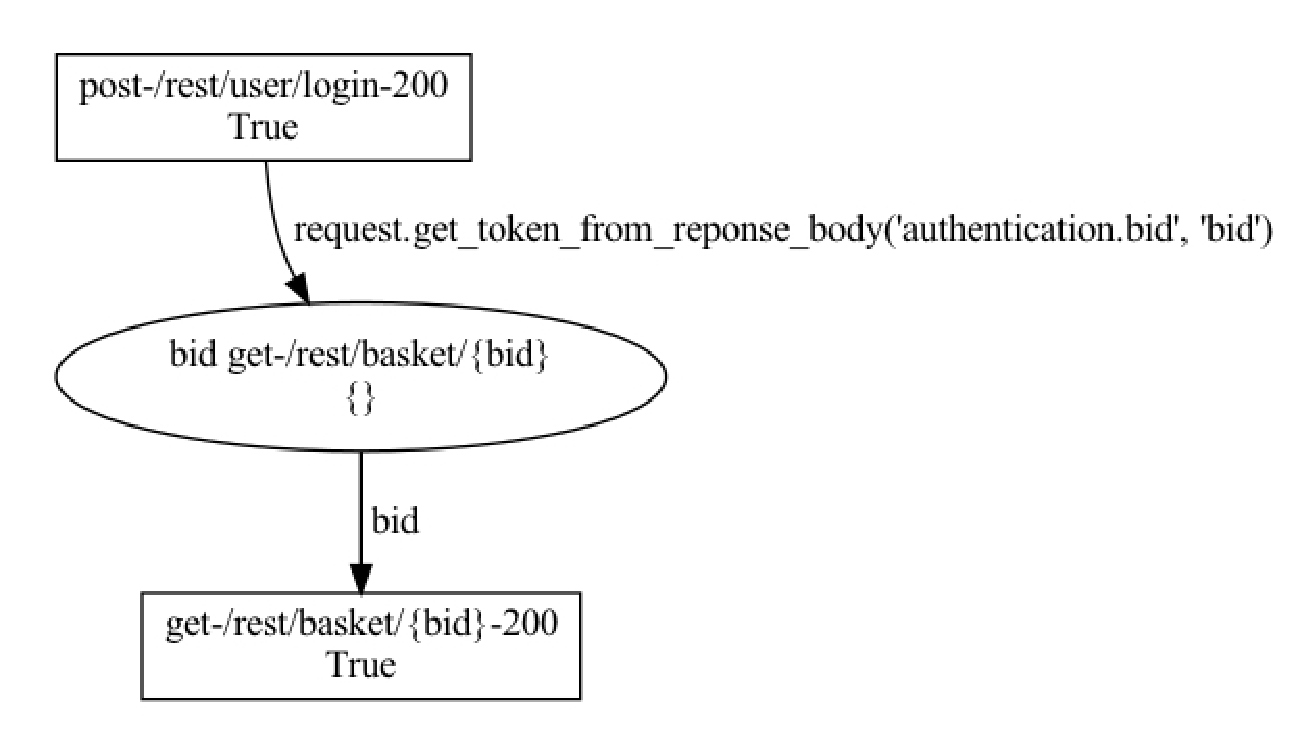
\includegraphics[width=1\columnwidth]{figures/SimpleJuiceShop-initial-state.png}
%    \caption{A simple WebAPI converted to Petri Net}
%    \label{fig:simplesWebAPIJuiceShopPetriNet-step-0}
%\end{figure}
%
%The next step is to replay the pairs request-response  on the model (this step is detailed in Section~\ref{sec:detecting_bola}).
%Considering the first pair request-response shown in Figure~\ref{fig:simplesWebAPIJuiceShop}, if we apply the \textit{Conformance  Checking Algorithm}, presented in \cite{10.1007/978-3-030-72610-2_33}, over the Petri Net shown in Figure~\ref{fig:simplesWebAPIJuiceShopPetriNet-step-0}, we obtain the Petri Net shown in Figure~\ref{fig:simplesWebAPIJuiceShopPetriNet-step1-step-2} a). Now, the place \textit{bid get-/rest/basket/{bid}} contains a token with the \textit{bid} equal to $1$ returned by the server and an identification of the client, in this case, an IP, but it could be the token, for example. Considering the second pair request-response shown in Figure~\ref{fig:simplesWebAPIJuiceShop} and applying 
%the \textit{Conformance  Checking Algorithm}, we get the Petri Net shown in Figure~\ref{fig:simplesWebAPIJuiceShopPetriNet-step1-step-2} b). The token that was in place \textit{bid get-/rest/basket/{bid}} was successfully consumed. In this example, we are just consuming the token. In the real world, we consume the token and the transition puts it back in place. This behavior is necessary to ensure the re-trigger capability of the second transition.
%
%On the other hand, considering now that the second pair request-response was composed of a request \textit{GET /basket/2}, 
%we could not trigger the second transition, as we would not have a token with \textit{bid} equal to $2$, generating an exception in the process, showing that was a violation in this dataflow. In the same way that if we try to apply the \textit{Conformance  Checking Algorithm} on the second pair request-response without have applied on the first pair request-response, we would receive an exception because we would not have tokens in place \textit{bid get-/rest/basket/{bid}}.
%
%\begin{figure}[!htp]
%    \center
%    \includegraphics[width=1\columnwidth]{figures/JuiceShop_Example-state-1-state2.png}
%    \caption{A simple WebAPI converted to Petri Net}
%    \label{fig:simplesWebAPIJuiceShopPetriNet-step1-step-2}
%\end{figure}

The excerpt of OpenAPI specification that we will use as running example is shown in Listing~\ref{lst:running_example_code} (see the appendix). In the rest of this paper, we use this running example to show how our model transformation approach can detect Broken Object Level Authorization (BOLA) attacks.
